\documentclass{standalone}
\usepackage{tikz}
\usetikzlibrary{patterns, positioning}
\usepackage[sfdefault]{ClearSans} %% option 'sfdefault' activates Clear Sans as the default text font
\usepackage[T1]{fontenc}

\begin{document}
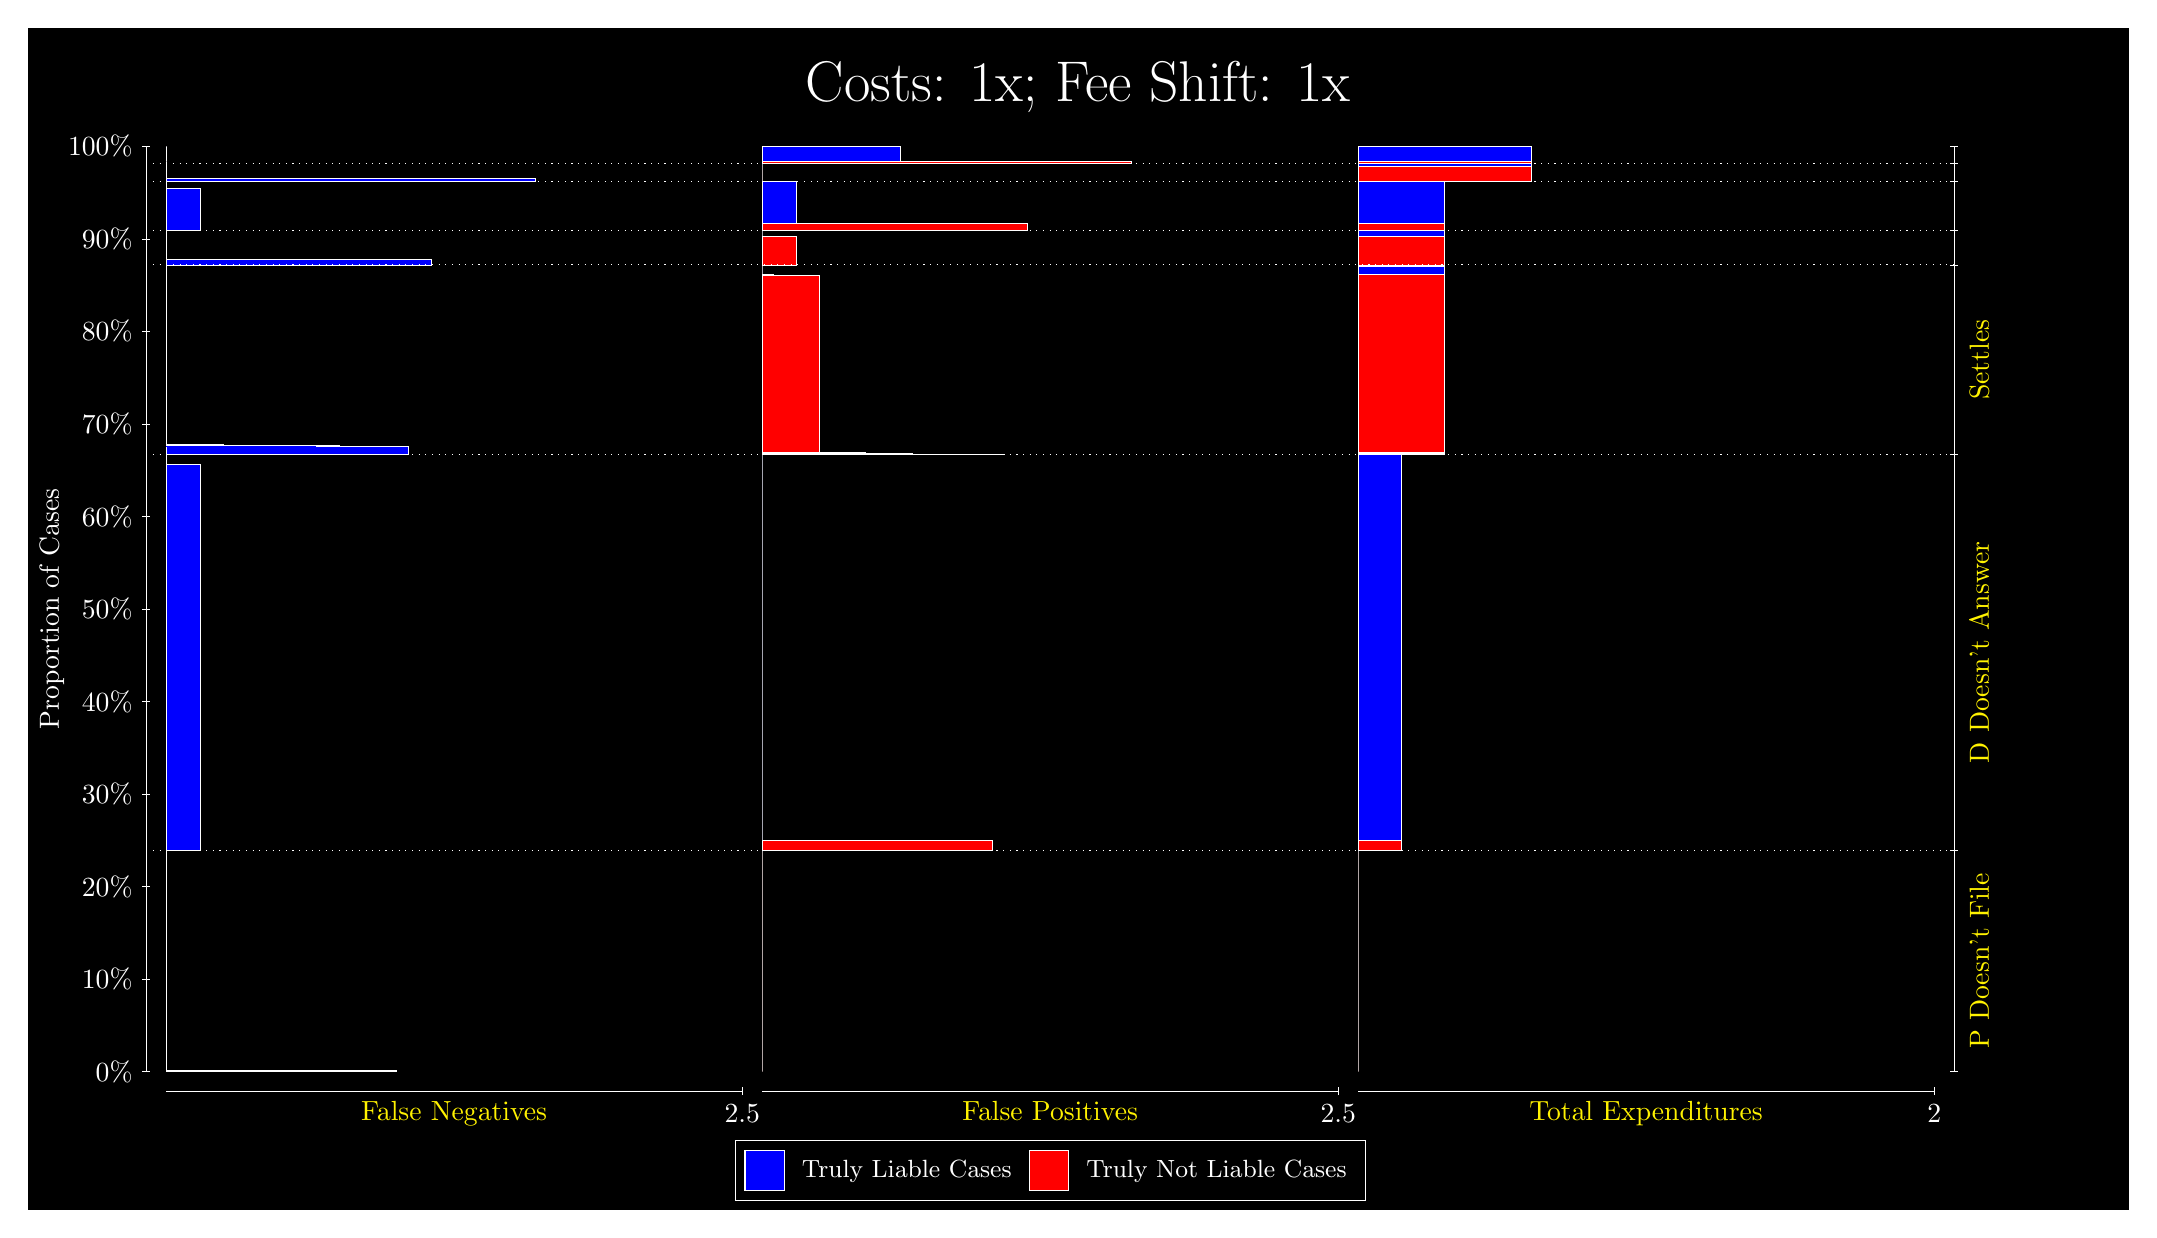
\begin{tikzpicture}
\draw[fill=black] (0,0) rectangle (26.667,15);
\draw[text=white] (0,13.5) rectangle (26.667,15) node[midway] {\huge Costs: 1x; Fee Shift: 1x};
\draw[white, very thin] (1.5,1.75) -- (1.5,13.5);
\node[rotate=90, text=white, anchor=center] at (0.3, 7.625) {Proportion of Cases};
\draw[white, very thin] (1.45,1.75) -- (1.55,1.75);
\node[text=white, anchor=east] at (1.45, 1.75) {0\%};
\draw[white, very thin] (1.45,2.925) -- (1.55,2.925);
\node[text=white, anchor=east] at (1.45, 2.925) {10\%};
\draw[white, very thin] (1.45,4.1) -- (1.55,4.1);
\node[text=white, anchor=east] at (1.45, 4.1) {20\%};
\draw[white, very thin] (1.45,5.275) -- (1.55,5.275);
\node[text=white, anchor=east] at (1.45, 5.275) {30\%};
\draw[white, very thin] (1.45,6.45) -- (1.55,6.45);
\node[text=white, anchor=east] at (1.45, 6.45) {40\%};
\draw[white, very thin] (1.45,7.625) -- (1.55,7.625);
\node[text=white, anchor=east] at (1.45, 7.625) {50\%};
\draw[white, very thin] (1.45,8.8) -- (1.55,8.8);
\node[text=white, anchor=east] at (1.45, 8.8) {60\%};
\draw[white, very thin] (1.45,9.975) -- (1.55,9.975);
\node[text=white, anchor=east] at (1.45, 9.975) {70\%};
\draw[white, very thin] (1.45,11.15) -- (1.55,11.15);
\node[text=white, anchor=east] at (1.45, 11.15) {80\%};
\draw[white, very thin] (1.45,12.325) -- (1.55,12.325);
\node[text=white, anchor=east] at (1.45, 12.325) {90\%};
\draw[white, very thin] (1.45,13.5) -- (1.55,13.5);
\node[text=white, anchor=east] at (1.45, 13.5) {100\%};

\draw[white, very thin] (24.457,1.75) -- (24.457,13.5);
\draw[white, very thin] (24.407,1.75) -- (24.507,1.75);
\node[anchor=west] at (24.407, 1.75) {};
\draw[white, very thin] (24.407,4.5581) -- (24.507,4.5581);
\node[anchor=west] at (24.407, 4.5581) {};
\draw[white, very thin] (24.407,9.5881) -- (24.507,9.5881);
\node[anchor=west] at (24.407, 9.5881) {};
\draw[white, very thin] (24.407,11.994) -- (24.507,11.994);
\node[anchor=west] at (24.407, 11.994) {};
\draw[white, very thin] (24.407,12.43) -- (24.507,12.43);
\node[anchor=west] at (24.407, 12.43) {};
\draw[white, very thin] (24.407,13.058) -- (24.507,13.058);
\node[anchor=west] at (24.407, 13.058) {};
\draw[white, very thin] (24.407,13.279) -- (24.507,13.279);
\node[anchor=west] at (24.407, 13.279) {};
\draw[white, very thin] (24.407,13.5) -- (24.507,13.5);
\node[anchor=west] at (24.407, 13.5) {};

\draw[white, very thin, fill=blue] (1.75,1.75) rectangle (4.6775,1.7689);
\draw[white, very thin, fill=red] (1.75,1.7689) rectangle (1.75,4.5581);
\draw[white, very thin, fill=blue] (1.75,4.5581) rectangle (2.1891,9.4598);
\draw[white, very thin, fill=red] (1.75,9.4598) rectangle (1.75,9.5881);
\draw[white, very thin, fill=blue] (1.75,9.5881) rectangle (4.8239,9.6934);
\draw[white, very thin, fill=blue] (1.75,9.6934) rectangle (4.5312,9.6945);
\draw[white, very thin, fill=blue] (1.75,9.6945) rectangle (4.2384,9.6959);
\draw[white, very thin, fill=blue] (1.75,9.6959) rectangle (3.9457,9.6974);
\draw[white, very thin, fill=blue] (1.75,9.6974) rectangle (3.6529,9.6995);
\draw[white, very thin, fill=blue] (1.75,9.6995) rectangle (3.3602,9.7002);
\draw[white, very thin, fill=blue] (1.75,9.7002) rectangle (3.0674,9.7016);
\draw[white, very thin, fill=blue] (1.75,9.7016) rectangle (2.7746,9.7024);
\draw[white, very thin, fill=blue] (1.75,9.7024) rectangle (2.4819,9.7139);
\draw[white, very thin, fill=red] (1.75,9.7139) rectangle (1.75,11.994);
\draw[white, very thin, fill=blue] (1.75,11.994) rectangle (5.1167,12.061);
\draw[white, very thin, fill=red] (1.75,12.061) rectangle (1.75,12.43);
\draw[white, very thin, fill=blue] (1.75,12.43) rectangle (2.1891,12.971);
\draw[white, very thin, fill=red] (1.75,12.971) rectangle (1.75,13.058);
\draw[white, very thin, fill=blue] (1.75,13.058) rectangle (6.4341,13.089);
\draw[white, very thin, fill=red] (1.75,13.089) rectangle (1.75,13.279);
\draw[white, very thin, fill=red] (1.75,13.279) rectangle (1.75,13.31);
\draw[white, very thin, fill=blue] (1.75,13.31) rectangle (1.75,13.5);
\draw[white, very thin, fill=red] (9.3189,1.75) rectangle (9.3189,4.5393);
\draw[white, very thin, fill=blue] (9.3189,4.5393) rectangle (9.3189,4.5581);
\draw[white, very thin, fill=red] (9.3189,4.5581) rectangle (12.246,4.6864);
\draw[white, very thin, fill=blue] (9.3189,4.6864) rectangle (9.3189,9.5881);
\draw[white, very thin, fill=red] (9.3189,9.5881) rectangle (12.393,9.5892);
\draw[white, very thin, fill=red] (9.3189,9.5892) rectangle (12.1,9.59);
\draw[white, very thin, fill=red] (9.3189,9.59) rectangle (11.807,9.5914);
\draw[white, very thin, fill=red] (9.3189,9.5914) rectangle (11.515,9.5921);
\draw[white, very thin, fill=red] (9.3189,9.5921) rectangle (11.222,9.599);
\draw[white, very thin, fill=red] (9.3189,9.599) rectangle (10.929,9.5991);
\draw[white, very thin, fill=red] (9.3189,9.5991) rectangle (10.929,9.6047);
\draw[white, very thin, fill=red] (9.3189,9.6047) rectangle (10.636,9.6099);
\draw[white, very thin, fill=red] (9.3189,9.6099) rectangle (10.344,9.6144);
\draw[white, very thin, fill=red] (9.3189,9.6144) rectangle (10.051,11.868);
\draw[white, very thin, fill=blue] (9.3189,11.868) rectangle (9.4652,11.879);
\draw[white, very thin, fill=blue] (9.3189,11.879) rectangle (9.3189,11.994);
\draw[white, very thin, fill=red] (9.3189,11.994) rectangle (9.758,12.363);
\draw[white, very thin, fill=blue] (9.3189,12.363) rectangle (9.3189,12.43);
\draw[white, very thin, fill=red] (9.3189,12.43) rectangle (12.686,12.518);
\draw[white, very thin, fill=blue] (9.3189,12.518) rectangle (9.758,13.058);
\draw[white, very thin, fill=red] (9.3189,13.058) rectangle (9.3189,13.249);
\draw[white, very thin, fill=blue] (9.3189,13.249) rectangle (9.3189,13.279);
\draw[white, very thin, fill=red] (9.3189,13.279) rectangle (14.003,13.31);
\draw[white, very thin, fill=blue] (9.3189,13.31) rectangle (11.075,13.5);
\draw[white, very thin, fill=red] (16.888,1.75) rectangle (16.888,4.5393);
\draw[white, very thin, fill=blue] (16.888,4.5393) rectangle (16.888,4.5581);
\draw[white, very thin, fill=red] (16.888,4.5581) rectangle (17.437,4.6864);
\draw[white, very thin, fill=blue] (16.888,4.6864) rectangle (17.437,9.5881);
\draw[white, very thin, fill=red] (16.888,9.5881) rectangle (17.986,9.5991);
\draw[white, very thin, fill=blue] (16.888,9.5991) rectangle (17.986,9.6158);
\draw[white, very thin, fill=red] (16.888,9.6158) rectangle (17.986,11.869);
\draw[white, very thin, fill=blue] (16.888,11.869) rectangle (17.986,11.974);
\draw[white, very thin, fill=red] (16.888,11.974) rectangle (17.986,11.99);
\draw[white, very thin, fill=blue] (16.888,11.99) rectangle (17.986,11.994);
\draw[white, very thin, fill=red] (16.888,11.994) rectangle (17.986,12.363);
\draw[white, very thin, fill=blue] (16.888,12.363) rectangle (17.986,12.43);
\draw[white, very thin, fill=red] (16.888,12.43) rectangle (17.986,12.518);
\draw[white, very thin, fill=blue] (16.888,12.518) rectangle (17.986,13.058);
\draw[white, very thin, fill=red] (16.888,13.058) rectangle (19.083,13.249);
\draw[white, very thin, fill=blue] (16.888,13.249) rectangle (19.083,13.279);
\draw[white, very thin, fill=red] (16.888,13.279) rectangle (19.083,13.31);
\draw[white, very thin, fill=blue] (16.888,13.31) rectangle (19.083,13.5);
\draw[white, dotted] (1.5,4.5581) -- (24.457,4.5581);
\draw[white, dotted] (1.5,9.5881) -- (24.457,9.5881);
\draw[white, dotted] (1.5,11.994) -- (24.457,11.994);
\draw[white, dotted] (1.5,12.43) -- (24.457,12.43);
\draw[white, dotted] (1.5,13.058) -- (24.457,13.058);
\draw[white, dotted] (1.5,13.279) -- (24.457,13.279);
\draw[white, very thin] (1.75,1.5) -- (9.0689,1.5);
\node[text=yellow, anchor=north] at (5.4094, 1.5) {False Negatives};
\draw[white, very thin] (9.0689,1.45) -- (9.0689,1.55);
\node[text=white, anchor=north] at (9.0689, 1.45) {2.5};

\draw[white, very thin] (9.3189,1.5) -- (16.638,1.5);
\node[text=yellow, anchor=north] at (12.978, 1.5) {False Positives};
\draw[white, very thin] (16.638,1.45) -- (16.638,1.55);
\node[text=white, anchor=north] at (16.638, 1.45) {2.5};

\draw[white, very thin] (16.888,1.5) -- (24.207,1.5);
\node[text=yellow, anchor=north] at (20.547, 1.5) {Total Expenditures};
\draw[white, very thin] (24.207,1.45) -- (24.207,1.55);
\node[text=white, anchor=north] at (24.207, 1.45) {2};

\node[text=yellow, centered, rotate=90] at (24.777, 3.1541) {P Doesn't File};
\node[text=yellow, centered, rotate=90] at (24.777, 7.0731) {D Doesn't Answer};
\node[text=yellow, centered, rotate=90] at (24.777, 10.791) {Settles};





\draw (12.978300999999998,1.5) node[draw=none] (baseCoordinate) {};
\begin{scope}[align=center]
        \matrix[scale=0.5, draw=white, below=0.5cm of baseCoordinate, nodes={draw}, column sep=0.1cm]{
            \node[rectangle, draw, minimum width=0.5cm, minimum height=0.5cm, fill=blue] {}; &
            \node[draw=none, font=\small, text=white] (B) {Truly Liable Cases}; &
            \node[rectangle, draw, minimum width=0.5cm, minimum height=0.5cm, fill=red] {}; &
            \node[draw=none, font=\small, text=white] (B) {Truly Not Liable Cases}; \\
            };
\end{scope}

\end{tikzpicture}
\end{document}